\chapter{Introduction}
\begin{itemize}
  \item Why does the safety of the medical devices, the software component in particular, so important?
  \item What is the difference between software specification and software requirement?
  \item What is the current practice to ensure software safety? 
  
  \item What's the problem with the current practice?
  \item Why do we need closed-loop verification?
  
  \item What is the benefit of using model-based design?
  \item Can we use model-based design for closed-loop verification?
  \item How much confidence can model-based closed-loop verification provide?
  \item How to validate a physiological model? Validated in what sense?
  \item How do we model the physiological environment that the device operates in? What are the challenges?
  \item What are the current practice for physiological modeling?
  \item What are the differences if we would like to use the models for closed-loop verification of medical devices?
	\item What are the different forms of model-based closed-loop verification?

    \item How to maintain safety guarantees through out the development process?
    \item What are possible problems that may arise during each steps?
    \item How can model-based design help during certification?
%     \item The pacemaker example

%     \begin{itemize}
%     	\item What are the steps of a possible model-based development process?
%         \item Heart Modeling

%         \begin{itemize}
%         	\item How to encode domain knowledge into the physiological models?
%         \end{itemize}
%         \item Model Validation
        
%         \begin{itemize}
%         	\item 
%         \end{itemize}
        
%         \item Abstract model checking
        
%           \begin{itemize}
%           	\item How to use models to cover environmental conditions specified in the physiological requirements, that the device may encounter?
%             \item What are the physiological requirements? What form should they be?
%             \item Can model checking find violations that testing cannot find?
%             \item What are the effects of adding new features? Can they disrupt the safety properties that the previous device hold?
%             \item What is the model complexity requirements for each physiological requirement? When and how to refine the environment model?
%             \item Exploring the whole state space sounds great. What are the limitations of model checking?
%           \end{itemize}
%         \item Model Simulation
        	
%           \begin{itemize}
%           	\item How can model simulation complement model checking?
%             \item How to model the interactions between the environment and the device?
           
%           \end{itemize}
        
%         \item Physical Testing
        
%           \begin{itemize}
%           	\item Is it necessary to make physical platform for the enviornment? What's the benefit?
%             \item Is there real-time requirements?
%             \item How to generate tests? What does closed-loop testing mean?
%             \item How much coverage can it achieve? How to quantify?
%           \end{itemize}
%         \item Traceability
        
%           \begin{itemize}
        
%             \item How to maintain safety confidence throughout the development process? 
%             \item What is the current practice?
%             \item Can it be automated?
%             \item How much confidence can it provide?
%           \end{itemize}
        
%         \item Certification
        
%           \begin{itemize}
%           	\item Can model-based closed-loop verification provide more safety guarantee than current practice? How much?
%           \end{itemize}
%     \end{itemize}
\end{itemize}


\begin{figure}[!b]
		\centering
		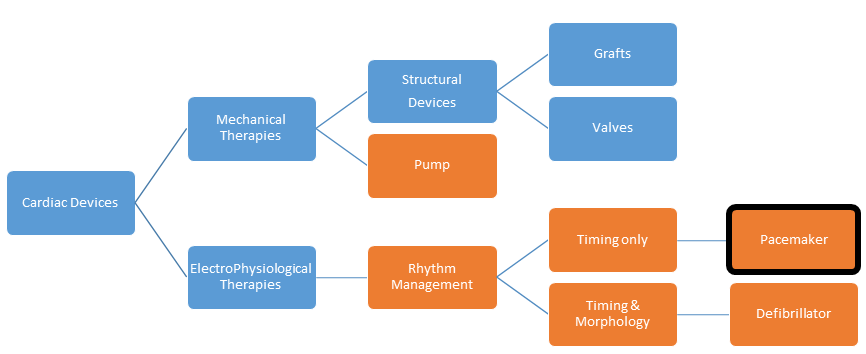
\includegraphics[width=0.8\textwidth]{figs/Fig1.png}
		%\vspace{-5pt}
		\caption{\small Scope of the survey}
		  %\vspace{-15pt}
		\label{fig:scope}
\end{figure}
\begin{figure}[!b]
		\centering
		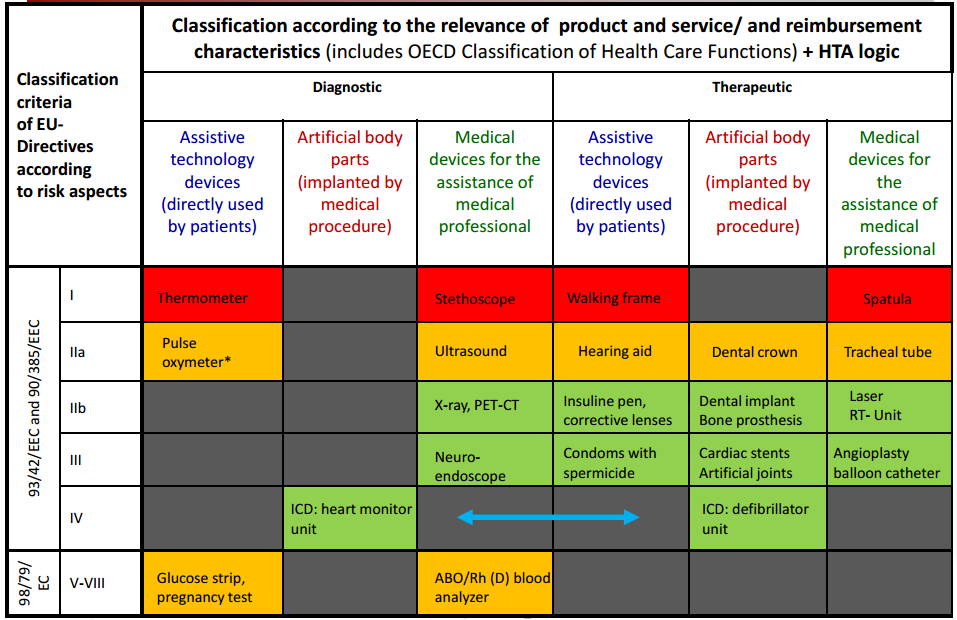
\includegraphics[width=0.5\textwidth]{figs/devices.png}
		%\vspace{-5pt}
		\caption{\small List of Cardiac devices}
		  %\vspace{-15pt}
		\label{fig:devices}
\end{figure}

\section{Medical Device Software Safety: Current Practice*}
\begin{itemize}
    \item What are the problems of the certification process?
    \item What are the safety proofs that the FDA receive?
    \item What is Open-loop Testing? What is the problem with it?
    \item What is the limitation of the clinical trials?
    
\end{itemize}

\section{Model-based Closed-loop Verification of Medical Device Software}
\begin{itemize}
	\item Can we replace real patient with models? What are the challenges? How much guarantee can we provide?
    \item In what forms can model-based closed-loop verification performed?
    \item What are the different requirements for the environment model in these forms?
\end{itemize}

\section{Traditional Physiological Modeling**}
\begin{itemize}
	\item Where are the applications of those physiological models?
    \item What are the key perspectives that the modeling should focus on?
    \item Can we use these models for model-based closed-loop verification?
    \item What are the difference between these applications?
\end{itemize}

\section{Modeling Perspectives**}
\begin{itemize}
	\item Complexity
    \item Generality
    \item Validation
\end{itemize}

\section{Model Applications}

\begin{itemize}
	\item Understanding physiological phenomena
	\item Closed-loop testing
	\item Closed-loop model checking
\end{itemize}
